\documentclass[11pt,a4paper]{article}

% ---------------------------------------------------------------------------
% Pacotes
% ---------------------------------------------------------------------------
\usepackage[T1]{fontenc}
\usepackage[utf8]{inputenc}
% Com o babel em português (ex.: Overleaf), a hifenização fica correta.
% Sem ele, a hifenização é desligada para evitar quebras com padrões do inglês.
\IfFileExists{portuges.ldf}{\usepackage[brazil]{babel}}{%
  \hyphenpenalty=10000 \exhyphenpenalty=10000
  \renewcommand{\figurename}{Figura}
  \renewcommand{\tablename}{Tabela}
  \renewcommand{\refname}{Referências}}
\usepackage{mathptmx}
\renewcommand{\ttdefault}{lmtt}
\usepackage[a4paper,top=1.8cm,bottom=1.8cm,left=1.8cm,right=1.8cm]{geometry}
\usepackage{amsmath}
\usepackage{graphicx}
\usepackage{adjustbox}
\usepackage[table]{xcolor}
\usepackage{tikz}
\usetikzlibrary{arrows.meta,positioning,calc}
\usepackage{array,tabularx}
\usepackage{caption,subcaption}
\usepackage{titlesec}
\usepackage{enumitem}
\usepackage{microtype}
\usepackage[hidelinks]{hyperref}

\emergencystretch=2em
\setlength{\parindent}{0pt}
\setlength{\parskip}{3pt}

% ---------------------------------------------------------------------------
% Estilo (modelo dos relatórios anteriores)
% ---------------------------------------------------------------------------
\definecolor{cabecalho}{RGB}{214,230,240}
\definecolor{azul}{RGB}{52,92,128}
\definecolor{pendente}{RGB}{200,0,0}

\titleformat{\section}{\Large\bfseries}{\thesection.}{0.35em}{}
\titleformat{\subsection}{\large\bfseries}{\thesubsection.}{0.35em}{}
\titlespacing*{\section}{0pt}{8pt plus 2pt minus 2pt}{3pt}
\titlespacing*{\subsection}{0pt}{5pt plus 2pt minus 1pt}{2pt}

\captionsetup{font={small,it},labelsep=endash,justification=centering,skip=4pt}
\captionsetup[sub]{font={footnotesize,it},skip=2pt}
\setlength{\textfloatsep}{8pt plus 2pt minus 2pt}
\setlength{\intextsep}{8pt plus 2pt minus 2pt}

\setlist{nosep,leftmargin=1.2em}
\arrayrulecolor{gray!60}
\newcolumntype{C}{>{\centering\arraybackslash}X}
\renewcommand{\arraystretch}{1.15}

% ---------------------------------------------------------------------------
% Campos a preencher
% ---------------------------------------------------------------------------
% Texto que ainda depende do grupo (busque por "\preencher").
\newcommand{\preencher}[1]{\textcolor{pendente}{[\textit{Preencher: #1}]}}

% \imagem{nome}{largura}{altura}{conteúdo esperado}
% Usa figuras/<nome>.png, .jpg ou .pdf se existir; caso contrário, desenha um
% espaço reservado do mesmo tamanho, para que a paginação não mude.
\newcommand{\imagem}[4]{%
  \IfFileExists{figuras/#1.png}{\includegraphics[width=#2,height=#3,keepaspectratio]{figuras/#1.png}}{%
  \IfFileExists{figuras/#1.jpg}{\includegraphics[width=#2,height=#3,keepaspectratio]{figuras/#1.jpg}}{%
  \IfFileExists{figuras/#1.pdf}{\includegraphics[width=#2,height=#3,keepaspectratio]{figuras/#1.pdf}}{%
  \tikz\node[draw=gray,dashed,minimum width=#2-0.4pt,minimum height=#3-0.4pt,
             text width=#2-10pt,align=center,inner sep=0pt,font=\scriptsize,text=gray]
            {\textbf{Inserir imagem:} \texttt{figuras/#1}\\#4};}}}}

% Ordem inferida (Figura 5b): índices de leitura das imagens, como na matriz de
% conectividade (metrics.json -> order e rejected).
\newcommand{\ordemInferida}{0,3,1,2,7,4,5,6,11,8,9,10}
\newcommand{\imagemIntrusa}{12}
\newcounter{nimagens}

\begin{document}

% ---------------------------------------------------------------------------
% Capa (não conta no limite de páginas)
% ---------------------------------------------------------------------------
\begin{titlepage}
\centering
\vspace*{1.5cm}
% Para usar o logotipo, salve-o como figuras/logo-unicamp.png (ou .jpg/.pdf).
\IfFileExists{figuras/logo-unicamp.png}{\includegraphics[width=6cm]{figuras/logo-unicamp.png}\par\vspace{1cm}}{}%
\IfFileExists{figuras/logo-unicamp.jpg}{\includegraphics[width=6cm]{figuras/logo-unicamp.jpg}\par\vspace{1cm}}{}%
\IfFileExists{figuras/logo-unicamp.pdf}{\includegraphics[width=6cm]{figuras/logo-unicamp.pdf}\par\vspace{1cm}}{}%
{\large\scshape Universidade Estadual de Campinas\par}
{\large\scshape Instituto de Computação\par}
\vspace{3.5cm}
{\large\bfseries Trabalho 1 -- Relatório Técnico\par}
{\large\bfseries MC919 Visão Computacional\par}
\vspace{1.2cm}
{\LARGE\bfseries Panoramas Automáticos a partir\\[2pt] de Imagens Fora de Ordem\par}
\vspace{0.4cm}
{\large\itshape Detecção, emparelhamento, ordenação, alinhamento e remoção de fantasmas\par}
\vspace{2.5cm}
{\bfseries Integrantes\par}
\vspace{4pt}
Bruno Medeiros Saback - 281746\\
Victor Luigi Roquetto - 250955\\
Lucas Souza Guimarães - 195948\\
Lucas Valadares Lima - 247025\par
\vspace{1cm}
\textbf{Professor:} Anderson Rocha\par
\vfill
2º semestre de 2026 -- Outubro de 2026\par
\end{titlepage}
\setcounter{page}{1}

\begin{center}\textbf{\large Resumo}\end{center}
\vspace{-6pt}
Este relatório apresenta um pipeline em Python e OpenCV que constrói panoramas automaticamente a partir
de uma pasta de imagens fora de ordem, sem uso de EXIF. O sistema extrai características com SIFT,
emparelha descritores com Brute Force e o ratio test de Lowe e estima, por RANSAC, a homografia de todos
os pares; a matriz de inliers define um grafo de vizinhança que rejeita intrusas e recupera a sequência
espacial. As imagens são alinhadas sobre uma árvore geradora de máxima confiança, refinadas por ajuste
global e compostas com feathering e remoção de fantasmas por detecção de pixels inconsistentes. Na cena
coletada, com 12 vistas de um quintal e uma intrusa, o pipeline rejeitou a intrusa, recuperou a sequência
mesmo com nomes aleatórios e gerou o panorama em projeção cilíndrica, pois o plano se mostrou inviável. Em
53 execuções que variam um parâmetro por vez, o ajuste global reduziu o erro mediano de consistência de
43,9 para 3,5~px, e o deghosting eliminou as cópias translúcidas da árvore em primeiro plano.

% ---------------------------------------------------------------------------
\section{Introdução e Visão Geral do Pipeline}
% ---------------------------------------------------------------------------
O objetivo é construir panoramas a partir de imagens parcialmente sobrepostas, recebidas fora de ordem e
misturadas a uma imagem de outra cena, sem intervenção manual. O pipeline segue a abordagem clássica de
costura baseada em características \cite{brown2007,szeliski2022}, implementada em Python com OpenCV,
NumPy e SciPy (Figura~\ref{fig:pipeline}). O comando \texttt{python -m panorama build <pasta>} produz o
panorama, as figuras intermediárias e um arquivo \texttt{metrics.json} com configuração, ordem inferida e
métricas.

O modelo geométrico é a homografia, válida para cenas aproximadamente planas ou para uma câmera que apenas
gira em torno do seu centro óptico. A leitura ignora o EXIF, inclusive a orientação, e os nomes dos
arquivos servem apenas como rótulos. As imagens são reduzidas a um maior lado fixo (1200~px por padrão e
600~px nos experimentos), escala à qual se referem os limiares e erros em pixels deste relatório.

\begin{figure}[!htb]
\centering
\resizebox{\linewidth}{!}{%
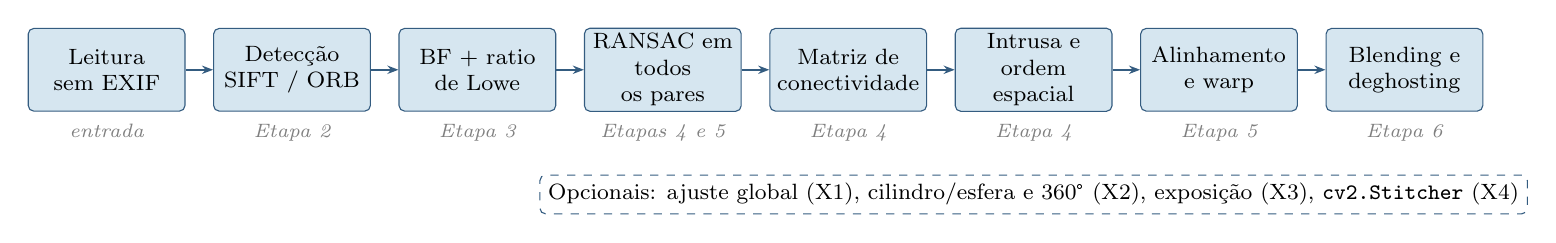
\begin{tikzpicture}[
    etapa/.style={draw=azul,fill=cabecalho,rounded corners=2pt,align=center,font=\footnotesize,
                  minimum height=1.05cm,text width=1.85cm,inner sep=2pt},
    rotulo/.style={font=\scriptsize\itshape,text=gray,below=1pt},
    seta/.style={-{Stealth[length=4pt]},thick,azul}]
  \node[etapa] (a) {Leitura\\sem EXIF};
  \node[etapa,right=0.35cm of a] (b) {Detecção\\SIFT / ORB};
  \node[etapa,right=0.35cm of b] (c) {BF + ratio\\de Lowe};
  \node[etapa,right=0.35cm of c] (d) {RANSAC em\\todos os pares};
  \node[etapa,right=0.35cm of d] (e) {Matriz de\\conectividade};
  \node[etapa,right=0.35cm of e] (f) {Intrusa e\\ordem espacial};
  \node[etapa,right=0.35cm of f] (g) {Alinhamento\\e warp};
  \node[etapa,right=0.35cm of g] (h) {Blending e\\deghosting};
  \foreach \u/\v in {a/b,b/c,c/d,d/e,e/f,f/g,g/h} \draw[seta] (\u) -- (\v);
  \node[rotulo] at (a.south) {entrada};
  \node[rotulo] at (b.south) {Etapa 2};
  \node[rotulo] at (c.south) {Etapa 3};
  \node[rotulo] at (d.south) {Etapas 4 e 5};
  \node[rotulo] at (e.south) {Etapa 4};
  \node[rotulo] at (f.south) {Etapa 4};
  \node[rotulo] at (g.south) {Etapa 5};
  \node[rotulo] at (h.south) {Etapa 6};
  \node[draw=azul,dashed,rounded corners=2pt,font=\footnotesize,align=center,inner sep=3pt]
       (x) at ($(d.south)!0.5!(h.south)+(0,-1.05)$)
       {Opcionais: ajuste global (X1), cilindro/esfera e 360° (X2), exposição (X3), \texttt{cv2.Stitcher} (X4)};
\end{tikzpicture}}
\caption{Visão geral do pipeline e correspondência com as etapas do enunciado.}
\label{fig:pipeline}
\end{figure}

% ---------------------------------------------------------------------------
\section{Coleta das Imagens e Metodologia Experimental}
\label{sec:metodologia}
% ---------------------------------------------------------------------------
\subsection{Coleta}
As imagens foram capturadas em um quintal residencial, ambiente externo, em 3 de outubro de 2026, com
iluminação natural e céu parcialmente nublado. \textbf{Dispositivo:} \preencher{câmera ou celular
utilizado e resolução original das fotos.} O conjunto (Anexo~A) tem 13 imagens: 12
vistas parcialmente sobrepostas, que varrem o quintal da fachada da casa, à esquerda, até a casa vizinha,
à direita, e uma imagem intrusa de um ambiente interno (vista 12). O elemento móvel é a folhagem da árvore
em primeiro plano, presente sobretudo nas vistas 0 a 3; as nuvens também se deslocam entre as capturas. A
cena tem grande variação de profundidade, com muro e plantas próximos da câmera e prédios distantes, o que
torna o alinhamento sensível a paralaxe.

\subsection{Metodologia experimental}
Como conjunto complementar, usaram-se as cinco imagens \emph{boat} do OpenCV \cite{opencv} (boat5),
renomeadas e sem intrusa. A configuração base (SIFT com até 2500 pontos, 600~px, ratio 0,75, RANSAC de
3~px, projeção cilíndrica com ajuste global, compensação de exposição, feathering e deghosting com limiar
30) foi variada um parâmetro por vez, em 25 variantes por conjunto, incluindo as sementes 7 e 101 além da
42. Com uma cópia do quintal com nomes aleatórios e o boat5 com ganhos de exposição artificiais, o pacote
\texttt{experiments} executou 53 execuções sequenciais, com uma thread. Sem homografias de referência, a geometria é avaliada pela
\emph{consistência em um suporte comum}: correspondências SIFT fixas e mais estritas (ratio 0,65, RANSAC
de 1,5~px e até 200 por par) são reprojetadas pela geometria final de cada variante, e reportam-se a
mediana e o percentil 95 (P95) do erro simétrico, em pixels a 600~px. A medida usa os mesmos pontos em
todas as variantes, mas não é ground truth e pode favorecer o SIFT, usado para construí-la. O tempo do
núcleo soma leitura, extração, emparelhamento, geometria e as duas composições (com e sem deghosting).

% ---------------------------------------------------------------------------
\section{Detecção e Extração de Características}
% ---------------------------------------------------------------------------
Foram implementados três detectores do OpenCV: SIFT \cite{lowe2004}, com descritor de 128 dimensões em
ponto flutuante e invariância a escala e rotação; ORB \cite{rublee2011}, com detector FAST orientado e
descritor binário; e AKAZE \cite{alcantarilla2013}, com espaço de escalas não linear e descritor binário.
Os keypoints são desenhados com um círculo proporcional à escala e um raio que indica a orientação
(Figura~\ref{fig:features}a e b). A Tabela~\ref{tab:detectores} compara os três em execuções completas
sobre o quintal, alterando apenas o detector.

O SIFT foi adotado como padrão: no quintal, gerou mais pares aceitos (34, contra 26 do ORB e 28 do AKAZE),
extraiu mais rápido e teve o menor P95 do erro (11,6~px, contra 26,0 e 28,5~px); o AKAZE teve a menor
mediana (2,96~px), mas cauda mais de duas vezes maior. A Figura~\ref{fig:features} sugere uma causa: o ORB
concentra os pontos na vegetação, enquanto o SIFT os distribui também pelo céu e pelas fachadas. No
boat5, os três aceitaram os mesmos 5 pares (medianas de 0,39 a 0,47~px), e o SIFT também extraiu mais
rápido (0,31~s, contra 1,43~s do ORB e 1,54~s do AKAZE). A conclusão vale para estes conjuntos, e não como
superioridade geral do SIFT.

\begin{table}[!htb]
\centering\small
\begin{tabularx}{\linewidth}{|C|C|C|C|C|C|C|}
\hline
\rowcolor{cabecalho}\textbf{Detector} & \textbf{Keypoints por imagem} & \textbf{Extração (s)} &
\textbf{Pares aceitos} & \textbf{Mediana (px)} & \textbf{P95 (px)} & \textbf{Tempo do núcleo (s)} \\ \hline
SIFT  & 1622 & 1,37 & 34 & 3,50 & 11,61 & 12,4 \\ \hline
ORB   & 2418 & 1,64 & 26 & 3,46 & 25,98 & 18,1 \\ \hline
AKAZE &  847 & 2,29 & 28 & 2,96 & 28,53 & 14,2 \\ \hline
\end{tabularx}
\caption{Detectores no quintal (13 imagens, 600~px, até 2500 pontos). Extração: tempo total nas 13
imagens; mediana e P95: erro de consistência.}
\label{tab:detectores}
\end{table}

\begin{figure}[!htb]
\centering
\begin{subfigure}[t]{0.235\linewidth}\centering
  \imagem{keypoints-sift}{\linewidth}{2.8cm}{\texttt{keypoints/sift/<i>.jpg}}
  \caption{SIFT}
\end{subfigure}\hfill
\begin{subfigure}[t]{0.235\linewidth}\centering
  \imagem{keypoints-orb}{\linewidth}{2.8cm}{\texttt{keypoints/orb/<i>.jpg}}
  \caption{ORB}
\end{subfigure}\hfill
\begin{subfigure}[t]{0.5\linewidth}\centering
  \imagem{matches-antes}{\linewidth}{2.8cm}{\texttt{matches/<i>\_<j>\_before.jpg}}
  \caption{Antes do ratio test}
\end{subfigure}\\[3pt]
\begin{subfigure}[t]{0.49\linewidth}\centering
  \imagem{matches-ratio}{\linewidth}{2.8cm}{\texttt{matches/<i>\_<j>\_ratio.jpg}}
  \caption{Após o ratio test e a unicidade}
\end{subfigure}\hfill
\begin{subfigure}[t]{0.49\linewidth}\centering
  \imagem{matches-inliers}{\linewidth}{2.8cm}{\texttt{matches/<i>\_<j>\_inliers.jpg}}
  \caption{Inliers do RANSAC}
\end{subfigure}
\caption{Keypoints da vista 5 (o círculo indica a escala e o raio, a orientação) e correspondências entre
as vistas 5 e 6 antes e depois da filtragem; no máximo 120 linhas são desenhadas.}
\label{fig:features}
\end{figure}

% ---------------------------------------------------------------------------
\section{Emparelhamento de Características}
% ---------------------------------------------------------------------------
Os descritores são emparelhados com o Brute Force Matcher do OpenCV, com distância L2 para o SIFT e de
Hamming para os descritores binários. Para cada descritor da imagem $i$, buscam-se os dois vizinhos mais
próximos na imagem $j$, com distâncias $d_1 \le d_2$, e o par é mantido se $d_1 < 0{,}75\,d_2$ (ratio test
de Lowe \cite{lowe2004}); em seguida, se vários pontos de $i$ apontam para o mesmo ponto de $j$, mantém-se
apenas o de menor distância.

Antes do ratio test (Figura~\ref{fig:features}c), muitas linhas cruzam a figura, pois a textura repetitiva
da vegetação produz vizinhos ambíguos. Após o ratio test e o RANSAC (Figuras~\ref{fig:features}d e e),
restam linhas aproximadamente paralelas, e 519 dos 587 pares que passaram no ratio test são inliers
(88\%). Correspondências erradas são eliminadas pelo RANSAC, pela verificação inversa de cada inlier
(Seção~\ref{sec:homografia}) e pela cobertura espacial mínima dos inliers (Seção~\ref{sec:ordem}). O
elemento móvel reduz o consenso: o par 1--3, com a árvore em primeiro plano nas duas vistas, tem a menor
taxa de inliers da Tabela~\ref{tab:pares} (43\%).

% ---------------------------------------------------------------------------
\section{Ordenação Automática das Imagens}
\label{sec:ordem}
% ---------------------------------------------------------------------------
\subsection{Matriz de conectividade e rejeição da intrusa}
Os arquivos são lidos em ordem alfabética apenas para receberem um índice; nomes, datas e EXIF não são
usados. Todos os $n(n-1)/2$ pares são avaliados, e o número de inliers do RANSAC de cada um preenche a
matriz de conectividade (Figura~\ref{fig:grafo}a). Um par se torna aresta do grafo de vizinhança quando
tem (i) ao menos 20 inliers, (ii) taxa de inliers (sobre os matches após o ratio test) de ao menos 0,3 e
(iii) fecho convexo dos inliers cobrindo ao menos 1\% da área de cada imagem; no quintal, 34 dos 78 pares
foram aceitos. A maior componente conexa do grafo é a cena, e as demais são rejeitadas; um empate de
tamanho interrompe a execução com uma mensagem explícita. A vista 12 teve no máximo 5 inliers com a cena
(com a vista 8), perto das 4 correspondências da amostra mínima de uma homografia e bem abaixo de 20;
ficou isolada e foi rejeitada (Figura~\ref{fig:grafo}b).

\subsection{Sequência a partir do grafo de vizinhança}
A imagem com maior soma de inliers nas arestas incidentes é a âncora, o referencial do mosaico, e a partir
dela constrói-se a árvore geradora de peso máximo (algoritmo de Prim, com peso igual ao número de
inliers). Pelo encadeamento das homografias da árvore, os centros das imagens são levados ao referencial
da âncora e ordenados ao longo do eixo principal (PCA) da sua distribuição; nas projeções curvas, usa-se o
azimute do eixo óptico de cada câmera, abrindo o ciclo no maior intervalo angular. A ordem inferida foi 0,
3, 1, 2, 7, 4, 5, 6, 11, 8, 9, 10, coerente com a varredura do panorama (Figura~\ref{fig:panorama}a), e a
árvore resultou em um caminho cujas arestas são exatamente os pares consecutivos dessa ordem. Sem
informação temporal, a ordem e a sua reversa são equivalentes. Com nomes aleatórios e bytes idênticos, a
sequência recuperada foi a mesma, a menos do sentido, e a mesma imagem foi rejeitada.

\begin{figure}[!htb]
\centering
\begin{subfigure}[b]{0.3\linewidth}\centering
  \imagem{conectividade}{\linewidth}{3.6cm}{\texttt{connectivity.png}}
  \caption{Matriz de conectividade}
\end{subfigure}\hfill
\begin{subfigure}[b]{0.66\linewidth}\centering
  \setcounter{nimagens}{0}%
  \adjustbox{max width=\linewidth}{%
  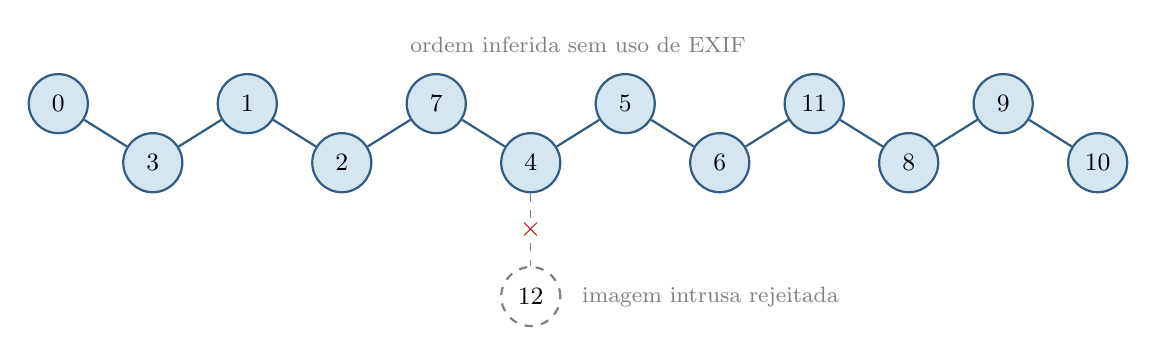
\begin{tikzpicture}[no/.style={circle,draw=azul,fill=cabecalho,thick,minimum size=0.75cm,
                                 inner sep=0pt,font=\small}]
    \foreach \v [count=\k] in \ordemInferida {
      \stepcounter{nimagens}
      \pgfmathsetmacro{\yy}{-0.75*mod(\k+1,2)}
      \node[no] (n\k) at (1.2*\k,\yy) {\v};
    }
    \pgfmathtruncatemacro{\total}{\value{nimagens}}
    \foreach \k in {2,...,\total} {
      \pgfmathtruncatemacro{\ant}{\k-1}
      \draw[thick,azul] (n\ant) -- (n\k);
    }
    \pgfmathtruncatemacro{\meio}{ceil(\total/2)}
    \pgfmathsetmacro{\xm}{0.6*(\total+1)}
    \node[font=\footnotesize,text=gray] at (\xm,0.75) {ordem inferida sem uso de EXIF};
    \node[no,dashed,fill=white,draw=gray] (x) at ($(n\meio)+(0,-1.7)$) {\imagemIntrusa};
    \draw[dashed,gray] (n\meio) -- node[fill=white,inner sep=1pt,text=pendente] {$\times$} (x);
    \node[right=4pt of x,font=\footnotesize,text=gray] {imagem intrusa rejeitada};
  \end{tikzpicture}}
  \caption{Grafo de vizinhança: ordem inferida e intrusa}
\end{subfigure}
\caption{A matriz de inliers define o grafo de vizinhança, do qual se obtém a ordem das imagens; a
intrusa, sem arestas válidas, é descartada. Os números são os índices de leitura das imagens.}
\label{fig:grafo}
\end{figure}

% ---------------------------------------------------------------------------
\section{Estimação de Homografia e Alinhamento}
\label{sec:homografia}
% ---------------------------------------------------------------------------
A homografia $H_{ij}$, que leva pixels da imagem $i$ para a imagem $j$, é estimada com
\texttt{cv2.findHomography} por RANSAC \cite{fischler1981}, com limiar de 3~px, confiança de 0,999 e até
5000 iterações. Cada inlier também precisa satisfazer a homografia inversa, com erro de até 6~px. Para cada
par utilizado são reportados a taxa de inliers, o erro de reprojeção médio $\bar{e}$ e o RMSE simétrico
sobre os $N$ inliers $(\mathbf{a}_k,\mathbf{b}_k)$, em que $\pi(\cdot)$ é a desomogeneização:
\begin{equation}
  \bar{e} = \frac{1}{N}\sum_{k=1}^{N}\big\|\pi(H_{ij}\mathbf{a}_k)-\mathbf{b}_k\big\|, \qquad
  \mathrm{RMSE} = \sqrt{\frac{1}{N}\sum_{k=1}^{N}
  \frac{\|\pi(H_{ij}\mathbf{a}_k)-\mathbf{b}_k\|^2 + \|\pi(H_{ij}^{-1}\mathbf{b}_k)-\mathbf{a}_k\|^2}{2}} .
\end{equation}
Nos 11 pares da árvore do quintal (Tabela~\ref{tab:pares}), a taxa de inliers variou de 43\% a 91\%, o
erro médio, de 0,59 a 1,31~px, e o RMSE simétrico ficou abaixo de 1,6~px.

\begin{table}[!htb]
\centering\footnotesize\setlength{\tabcolsep}{3pt}
\begin{minipage}[t]{0.495\linewidth}\centering
\begin{tabularx}{\linewidth}[t]{|C|C|C|C|C|C|}
\hline
\rowcolor{cabecalho}\textbf{Par} & \textbf{Matches} & \textbf{Inliers} & \textbf{Taxa (\%)} &
\textbf{Erro (px)} & \textbf{RMSE (px)} \\ \hline
0--3  & 336 & 252 & 75,0 & 0,69 & 0,88 \\ \hline
1--2  & 501 & 305 & 60,9 & 1,01 & 1,20 \\ \hline
1--3  & 254 & 110 & 43,3 & 0,59 & 0,74 \\ \hline
2--7  & 341 & 238 & 69,8 & 0,99 & 1,21 \\ \hline
4--5  & 494 & 450 & 91,1 & 1,00 & 1,21 \\ \hline
4--7  & 369 & 281 & 76,2 & 1,26 & 1,50 \\ \hline
\end{tabularx}
\end{minipage}\hfill
\begin{minipage}[t]{0.495\linewidth}\centering
\begin{tabularx}{\linewidth}[t]{|C|C|C|C|C|C|}
\hline
\rowcolor{cabecalho}\textbf{Par} & \textbf{Matches} & \textbf{Inliers} & \textbf{Taxa (\%)} &
\textbf{Erro (px)} & \textbf{RMSE (px)} \\ \hline
5--6  & 587 & 519 & 88,4 & 1,20 & 1,42 \\ \hline
6--11 & 644 & 430 & 66,8 & 1,08 & 1,31 \\ \hline
8--9  & 622 & 494 & 79,4 & 1,29 & 1,45 \\ \hline
8--11 & 556 & 416 & 74,8 & 1,31 & 1,55 \\ \hline
9--10 & 547 & 463 & 84,6 & 1,27 & 1,50 \\ \hline
\end{tabularx}
\end{minipage}
\caption{Pares da árvore geradora do quintal: matches após o ratio test, inliers, taxa de inliers, erro de
reprojeção médio e RMSE simétrico da homografia do par (px a 600~px).}
\label{tab:pares}
\end{table}

O alinhamento encadeia as homografias da árvore: sendo $T_i$ a transformação da imagem $i$ para o
referencial da âncora ($T_{\text{âncora}} = I$), cada imagem $j$ ligada na árvore a uma imagem $i$ já
alinhada recebe
\begin{equation}
  T_j = T_i \, H_{ij}^{-1} .
\end{equation}
No plano, as imagens são projetadas com \texttt{cv2.warpPerspective} em um canvas que contém os cantos
transformados de todas elas, com máscaras de validade que distinguem pixels pretos da cena de regiões sem
dados; se alguma imagem cruza o infinito ou o canvas excede o limite de área, a execução é interrompida.
Isso ocorreu nos dois conjuntos: no quintal, a projeção plana da vista 0 cruza o infinito, e no boat5 o
canvas chegaria a cerca de 8000$\times$3700~px. Por isso, os resultados usam a projeção cilíndrica, com as
homografias convertidas em rotações e projetadas com \texttt{cv2.remap} (Seção~\ref{sec:extras});
a Figura~\ref{fig:progressivo} mostra o alinhamento progressivo.

\begin{figure}[!htb]
\centering
\begin{subfigure}[t]{0.325\linewidth}\centering
  \imagem{progressivo-1}{\linewidth}{1.9cm}{\texttt{progressive/002.jpg}}
  \caption{Duas imagens}
\end{subfigure}\hfill
\begin{subfigure}[t]{0.325\linewidth}\centering
  \imagem{progressivo-2}{\linewidth}{1.9cm}{\texttt{progressive/006.jpg}}
  \caption{Seis imagens}
\end{subfigure}\hfill
\begin{subfigure}[t]{0.325\linewidth}\centering
  \imagem{progressivo-3}{\linewidth}{1.9cm}{\texttt{progressive/012.jpg}}
  \caption{Todas as imagens}
\end{subfigure}
\caption{Alinhamento progressivo: cada imagem é acrescentada ao mosaico seguindo a ordem inferida.}
\label{fig:progressivo}
\end{figure}

% ---------------------------------------------------------------------------
\section{Composição, Blending e Remoção de Fantasmas}
% ---------------------------------------------------------------------------
\subsection{Composição e blending}
A composição é incremental e segue a ordem inferida: cada imagem projetada $B$ é combinada ao mosaico
acumulado $A$. No feathering, o peso de cada fonte depende da distância do pixel à borda da sua região
válida ($d_A$ e $d_B$), calculada por transformada de distância:
\begin{equation}
  I = \alpha A + (1-\alpha) B, \qquad \alpha = \frac{d_A}{d_A + d_B} .
\end{equation}
Como alternativa, o blending multibanda \cite{burt1983} mistura cada nível de pirâmides laplacianas (até 5
níveis) com a versão gaussiana correspondente de $\alpha$, suavizando as baixas frequências em faixas
largas e preservando os detalhes.

\subsection{Remoção de fantasmas}
Um objeto que se move entre as capturas aparece em posições distintas nas duas fontes, e a média gera
cópias translúcidas (fantasmas). O pipeline marca, na sobreposição, os pixels cuja diferença absoluta média
entre os canais BGR das duas fontes excede 30 (escala 0--255), dilata a máscara em 5~px, descarta
componentes conexas menores que 25~px e atribui a cada componente uma única fonte, a de maior distância
média à própria borda, copiada diretamente mesmo no multibanda. Os mosaicos com e sem deghosting são
gerados na mesma execução e comparados em um recorte ampliado 2$\times$.

No quintal, sem deghosting, a árvore aparece em várias cópias translúcidas, pois a folhagem muda de
posição entre as vistas; com deghosting, ela fica nítida (Figura~\ref{fig:panorama}b). Com limiar 15, o
recorte é semelhante; com 60, surgem descontinuidades entre fontes no céu e no prédio ao fundo. A detecção
não é específica do objeto móvel: a seleção de fonte atingiu 69\% da área válida com limiar 30 (82\% com
15 e 45\% com 60), pois paralaxe, nuvens e brilho também geram inconsistências. Em um controle sintético
com fundo conhecido (15 condições), o método eliminou a mistura nos casos de alto contraste, mas só
recuperou o fundo quando a fonte escolhida não continha o objeto: o erro em relação ao fundo caiu de 34,9
para 0 no caso favorável e subiu de 58,3 para 93,2 no adverso. Com baixo contraste, apenas o limiar 15
detectou o objeto.

\subsection{Avaliação do resultado}
Na metade esquerda do panorama (Figura~\ref{fig:panorama}a), a borda superior do muro, os prédios ao fundo
e a fiação seguem sem quebras, e a árvore aparece uma única vez. Na metade direita, onde o muro e a casa
vizinha estão mais próximos da câmera, há degraus visíveis na borda do muro e no beiral do telhado, além
de recortes retangulares no céu e na fachada branca, causados pela troca de fonte do deghosting. A borda
ondulada do canvas reflete pequenas diferenças de inclinação entre as vistas. Quantitativamente, o erro de
consistência teve mediana de 3,50~px e P95 de 11,6~px, o erro médio de reprojeção nos pares usados após o
ajuste foi de 2,90~px, 84\% do canvas é coberto por dados e a diferença fotométrica média nas
correspondências fixas foi de 9,4 níveis de cinza.

\begin{figure}[!htb]
\centering
\begin{subfigure}[t]{\linewidth}\centering
  \imagem{panorama}{\linewidth}{4.6cm}{\texttt{panorama.png}}
  \caption{Panorama final: projeção cilíndrica, ajuste global, compensação de exposição, feathering e
  deghosting}
\end{subfigure}\\[4pt]
\begin{subfigure}[t]{0.5\linewidth}\centering
  \imagem{deghost}{\linewidth}{3.3cm}{\texttt{deghost\_comparison.png}}
  \caption{Recorte ampliado 2$\times$, sem (esquerda) e com (direita) remoção de fantasmas}
\end{subfigure}\hfill
\begin{subfigure}[t]{0.48\linewidth}\centering
  \imagem{stitcher}{\linewidth}{3.3cm}{\texttt{reference/panorama.png}}
  \caption{Referência \texttt{cv2.Stitcher} com as imagens aceitas}
\end{subfigure}
\caption{Resultado da composição no quintal, efeito da remoção de fantasmas e referência pronta do OpenCV.}
\label{fig:panorama}
\end{figure}

% ---------------------------------------------------------------------------
\section{Extras}
\label{sec:extras}
% ---------------------------------------------------------------------------
\subsection{Ajuste global dos parâmetros (X1)}
O encadeamento par a par acumula erros e ignora as arestas fora da árvore. O ajuste global refina todas as
transformações (com a âncora fixa) usando \texttt{scipy.optimize.least\_squares} sobre os resíduos de
reprojeção direta e inversa de inliers amostrados, com perda robusta soft-L1. No plano, otimiza 8
parâmetros de homografia por imagem; nas projeções curvas, usa o modelo de rotação pura \cite{brown2007},
com 3 parâmetros por câmera, um fator focal comum e $H_{ij} = K_j R_j^{\top} R_i K_i^{-1}$. A solução só é
aceita se não aumentar o erro, e atalhos (arestas fora da árvore) com erro mediano acima de
$\max(15~\text{px};\,8\%\text{ da largura})$ sob as transformações iniciais são descartados antes, para
evitar laços falsos.

No quintal, o encadeamento par a par teve mediana de 43,9~px e P95 de 138~px, com prédios e telhados
visivelmente duplicados; com o ajuste global, os valores caíram para 3,5 e 11,6~px
(Tabela~\ref{tab:variantes}). Parte do ganho vem da estimativa do foco, que passou de 0,9 para 0,683 da
largura (campo de visão horizontal de cerca de 72°). O foco inicial também afeta a verificação de atalhos:
com 0,9, 23 dos 34 pares aceitos foram descartados e o ajuste usou só as 11 arestas da árvore; com 0,6,
apenas 4 foram descartados, o ajuste usou 30 arestas e a mediana caiu para 2,23~px (P95 de 6,8~px). No
boat5, o padrão se repete: 42,7~px par a par contra 0,40~px com ajuste.

\subsection{Projeções cilíndrica e esférica e panorama de 360° (X2)}
Cada câmera é descrita por uma rotação $R_i$, a rotação mais próxima (via SVD) de $K_j^{-1}H_{ij}K_i$, e por
intrínsecos $K$ com foco proporcional à largura, sem EXIF. Um raio $(x,y,z)$ é mapeado para
$\theta = \operatorname{atan2}(x,z)$ e $v = y/\sqrt{x^2+z^2}$ no cilindro, ou
$\phi = \operatorname{atan2}(y,\sqrt{x^2+z^2})$ na esfera, com mapeamento inverso via \texttt{cv2.remap}.
No modo 360°, o canvas cobre exatamente $2\pi$ de longitude, tratada de forma periódica no blending.
Cilindro e esfera usam as mesmas rotações e tiveram o mesmo erro geométrico; diferem na deformação
vertical do canvas.

\subsection{Compensação de exposição (X3)}
Ganhos escalares $g_i$ são estimados pela luminância suavizada nos inliers, sem pixels escuros ou
saturados: com a mediana de $\log(I_j/I_i)$ em cada aresta, resolve-se por mínimos quadrados
$\log g_i - \log g_j = \log(I_j/I_i)$, com o ganho da âncora fixo em 1 e os demais em $[0{,}4;\,2{,}5]$. Os
ganhos são aplicados antes do deghosting. No boat5 com ganhos artificiais conhecidos (de 0,65 a 1,2), a
diferença fotométrica média nas correspondências caiu de 41,5 para 4,2 níveis, e a área marcada pelo
deghosting, de 56\% para 7\%: sem compensação, diferenças de exposição seriam tomadas como movimento. No
quintal, a diferença caiu de 11,5 para 9,4 níveis.

\subsection{Sensibilidade e comparação com o \texttt{cv2.Stitcher} (X4)}
No quintal (Tabela~\ref{tab:variantes}), ratio e RANSAC mais estritos reduziram a mediana e o P95, valores
permissivos aumentaram a cauda do erro, e 900~px mais que dobraram o tempo sem reduzir o erro; no boat5, as
variantes ficaram entre 0,39 e 0,45~px. O multibanda não altera a geometria e aumentou o tempo em cerca de
26\%, e as três sementes produziram métricas geométricas idênticas (12,40~$\pm$~0,02~s).

O \texttt{cv2.Stitcher}, com as mesmas imagens redimensionadas, concluiu nas três sementes, tanto com as
imagens aceitas quanto com as 13 entradas, incluindo a intrusa. Seu panorama
(Figura~\ref{fig:panorama}c) tem emendas mais suaves e céu sem recortes, mas não inclui a fachada da casa à
esquerda. O tempo médio foi de 6,3~s, contra 12,4~s do núcleo próprio, que faz duas composições e registra
diagnósticos; os escopos, portanto, não são idênticos.

\begin{table}[!htb]
\centering\footnotesize
\begin{tabularx}{\linewidth}{|>{\raggedright\arraybackslash}p{5.2cm}|C|C|C|C|C|}
\hline
\rowcolor{cabecalho}\textbf{Variante} & \textbf{Quintal: mediana (px)} & \textbf{Quintal: P95 (px)} &
\textbf{Quintal: núcleo (s)} & \textbf{Boat5: mediana (px)} & \textbf{Boat5: P95 (px)} \\ \hline
Base: cilindro, ajuste global, ganho    & 3,50 & 11,61 & 12,4 & 0,40 & 2,85 \\ \hline
Alinhamento par a par                   & 43,86 & 138,18 & 13,6 & 42,67 & 77,22 \\ \hline
Projeção esférica                       & 3,50 & 11,61 & 12,0 & 0,40 & 2,85 \\ \hline
Projeção plana (com e sem ajuste)       & falhou & -- & -- & falhou & -- \\ \hline
Foco inicial 0,6 / 1,2                  & 2,23 / 3,50 & 6,77 / 11,61 & 12,7 / 12,4 & 0,40 / 0,41 & 2,85 / 2,85 \\ \hline
Ratio 0,60 / 0,85                       & 3,00 / 3,83 & 7,92 / 28,59 & 14,6 / 22,6 & 0,40 / 0,39 & 2,42 / 2,44 \\ \hline
RANSAC 1,5 / 6~px                       & 2,68 / 3,86 & 9,22 / 13,45 & 13,4 / 12,6 & 0,40 / 0,45 & 2,78 / 2,31 \\ \hline
Limite SIFT 1000 / 5000 pontos          & 3,88 / 3,50 & 19,53 / 11,61 & 9,7 / 12,3 & 0,40 / 0,40 & 2,85 / 2,85 \\ \hline
Maior lado 400 / 900~px                 & 3,71 / 4,47 & 13,89 / 28,78 & 5,3 / 26,8 & 0,40 / 0,43 & 2,63 / 2,32 \\ \hline
\end{tabularx}
\caption{Erro de consistência (px a 600~px) e tempo do núcleo, alterando um parâmetro por vez em relação
à base; nas linhas com dois valores, cada um corresponde a uma das opções.}
\label{tab:variantes}
\end{table}

% ---------------------------------------------------------------------------
\section{Discussão e Conclusão}
% ---------------------------------------------------------------------------
O pipeline executou todo o fluxo sem intervenção manual: rejeitou a intrusa, recuperou a sequência das 12
vistas, inclusive com nomes aleatórios, e produziu um panorama cilíndrico com erro mediano de consistência
de 3,5~px. O ajuste global foi a etapa de maior impacto na geometria, o foco inicial influenciou quais
arestas entram no ajuste e critérios de emparelhamento mais estritos reduziram a cauda do erro. O
deghosting eliminou as cópias translúcidas da árvore, mas o controle sintético mostra que eliminar a
transparência não garante recuperar o fundo. Testes automatizados com cenas sintéticas e gabarito
verificam ainda a rejeição da intrusa, a independência entre nomes e ordem e o fechamento em 360°.

As principais limitações decorrem das hipóteses do modelo: (i) a homografia pressupõe cena plana ou
rotação pura, e a paralaxe perto da câmera explica os degraus na metade direita do panorama; (ii) a
ordenação supõe uma varredura em faixa única, e a rejeição da intrusa supõe que a cena seja a maior
componente do grafo; (iii) o deghosting não identifica semanticamente o objeto móvel e cria recortes
visíveis; e (iv) a exposição é corrigida por um ganho escalar, sem balanço de branco ou vinheta.

\begin{thebibliography}{9}
\footnotesize
\setlength{\itemsep}{0pt}
\bibitem{lowe2004} D. G. Lowe. Distinctive image features from scale-invariant keypoints. \textit{IJCV},
60(2):91--110, 2004.
\bibitem{rublee2011} E. Rublee, V. Rabaud, K. Konolige e G. Bradski. ORB: an efficient alternative to SIFT
or SURF. \textit{ICCV}, p. 2564--2571, 2011.
\bibitem{alcantarilla2013} P. F. Alcantarilla, J. Nuevo e A. Bartoli. Fast explicit diffusion for
accelerated features in nonlinear scale spaces. \textit{BMVC}, 2013.
\bibitem{fischler1981} M. A. Fischler e R. C. Bolles. Random sample consensus: a paradigm for model
fitting with applications to image analysis and automated cartography. \textit{Commun. ACM},
24(6):381--395, 1981.
\bibitem{brown2007} M. Brown e D. G. Lowe. Automatic panoramic image stitching using invariant features.
\textit{IJCV}, 74(1):59--73, 2007.
\bibitem{burt1983} P. J. Burt e E. H. Adelson. A multiresolution spline with application to image
mosaics. \textit{ACM Trans. Graphics}, 2(4):217--236, 1983.
\bibitem{szeliski2022} R. Szeliski. \textit{Computer Vision: Algorithms and Applications}. 2ª ed.,
Springer, 2022.
\bibitem{opencv} OpenCV. Tutorial da API de stitching e imagens \texttt{opencv\_extra/testdata/stitching}.
\url{https://docs.opencv.org/4.x/d8/d19/tutorial_stitcher.html}.
\end{thebibliography}

% ---------------------------------------------------------------------------
% Anexo (não conta no limite de páginas)
% ---------------------------------------------------------------------------
\clearpage
\setcounter{page}{1}
\renewcommand{\thepage}{A\arabic{page}}
\section*{Anexo A -- Imagens Coletadas}
As 13 imagens de entrada do quintal, na ordem de leitura (alfabética pelo nome do arquivo), que não
corresponde à ordem de captura. Os índices são os mesmos usados nas figuras e tabelas do relatório; a
vista 12 é a imagem intrusa, de um ambiente interno.

\begin{figure}[!htb]
\centering
\imagem{anexo-fotos}{\linewidth}{0.8\textheight}{Grade com as 13 imagens de entrada e seus índices}
\caption{Imagens de entrada do quintal; a vista 12 é a intrusa.}
\label{fig:entradas}
\end{figure}

\end{document}
